%%*****************************************************************************
%% $Id$
%%*****************************************************************************
%% @author Gerd Neugebauer
%%-----------------------------------------------------------------------------
\section{Modelling: Jude}

Jude is a UML modeller written in Java. It is distributed in a
community edition for free use. Currently the version 1.6.2 is
available from \url{http://www.esm.jp/jude-web/index.html}. 
\begin{figure}[thp]
  \centering
  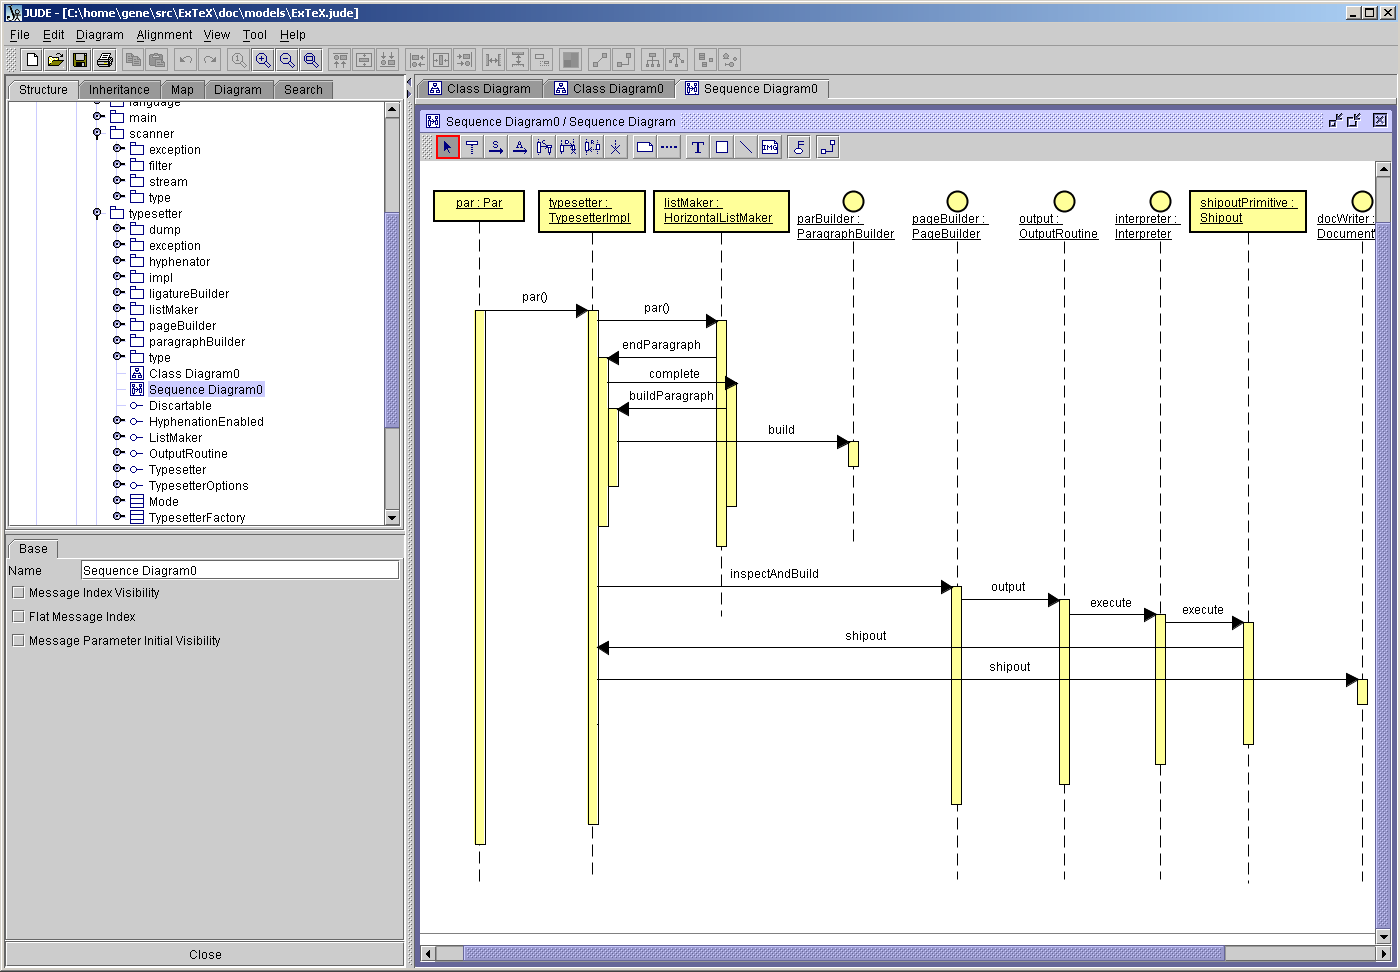
\includegraphics[width=\textwidth]{image/jude-seq}
  \caption{Jude}\label{fig:jude}
\end{figure}

Jude should be used for any situations where UML diagrams are needed.
A screenshot of Jude can be seen in figure~\ref{fig:jude}.

Models for \ExTeX\ should be placed in the directory \File{doc/models}.

